%%%%%%%%%%%%%%%%%%%%%%%%%%%%%%%%%%%%%%%%%%%%%%%%%%%%%%%%%%%%%
%% HEADER
%%%%%%%%%%%%%%%%%%%%%%%%%%%%%%%%%%%%%%%%%%%%%%%%%%%%%%%%%%%%%
\documentclass[a4paper,twoside,11pt]{article}

%% Language %%%%%%%%%%%%%%%%%%%%%%%%%%%%%%%%%%%%%%%%%%%%%%%%%
\usepackage[T1]{fontenc}

%\usepackage[ansinew]{inputenc}
\usepackage[utf8]{inputenc}	%supports Umlaute
\usepackage{german, ngerman}
\usepackage{color}

\usepackage{lmodern} %Type1-font for non-english texts and characters

%% Packages for Graphics & Figures %%%%%%%%%%%%%%%%%%%%%%%%%%
\usepackage{graphicx} %%For loading graphic files
\usepackage{multicol}

%% Math Packages %%%%%%%%%%%%%%%%%%%%%%%%%%%%%%%%%%%%%%%%%%%%
\usepackage{amsmath}
\usepackage{amsthm}
\usepackage{amsfonts}
\usepackage{amssymb}

%% Line Spacing %%%%%%%%%%%%%%%%%%%%%%%%%%%%%%%%%%%%%%%%%%%%%
\usepackage[parfill]{parskip}    % Activate to begin paragraphs with an empty line rather than an indent

%% Other Packages %%%%%%%%%%%%%%%%%%%%%%%%%%%%%%%%%%%%%%%%%%%
\usepackage{a4wide} %%Smaller margins = more text per page.
\usepackage{fancyhdr} %%Fancy headings

%%%%%%%%%%%%%%%%%%%%%%%%%%%%%%%%%%%%%%%%%%%%%%%%%%%%%%%%%%%%%
%% DOCUMENT
%%%%%%%%%%%%%%%%%%%%%%%%%%%%%%%%%%%%%%%%%%%%%%%%%%%%%%%%%%%%%
\begin{document}

\pagestyle{fancyplain}

%% Title Page %%%%%%%%%%%%%%%%%%%%%%%%%%%%%%%%%%%%%%%%%%%%%%%
\title{Parallel Programming Assignment \#1} 
\author{Marcel Karsten,\\ Patrick Lorenz,\\ Richard Klemm}
\date{Due: Thursday, 03th January 2012} %%If commented, the current date is used.
\maketitle

%% Header on top of every page (yes, also on the title page!)
\rhead{Parallel Programming - TU Berlin, SS/12}
\lhead{}
\renewcommand{\headrulewidth}{0px}


%%%%%%%%%%%%%%%%%%%%%%%%%%%%%%%%%%%%%%%%%%%%%%%%%%%%%%%%%%%%%

\section{Exercise 3}
\hspace{2em}\textbf{(a)}
\begin{figure}[!htbp]
    \begin{center}
        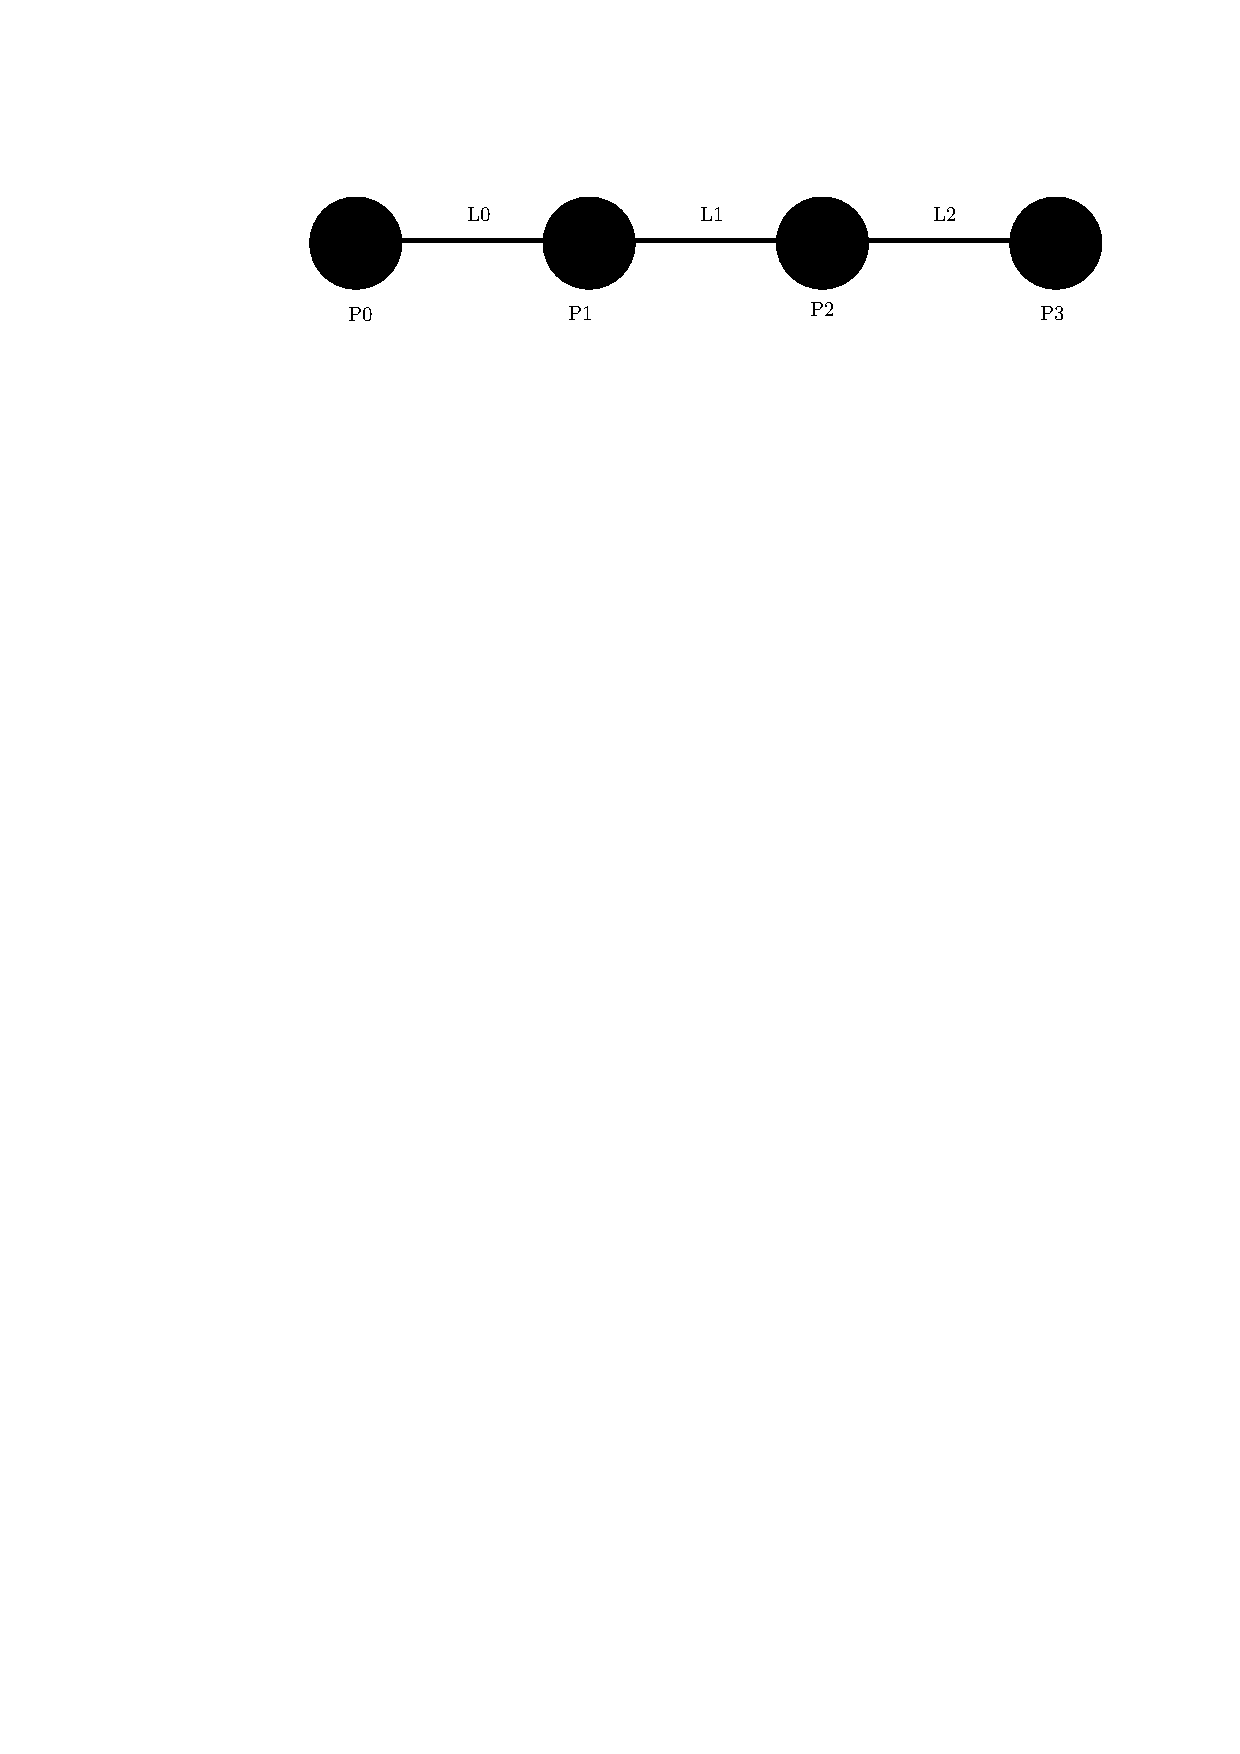
\includegraphics[scale=1]{3a_1.pdf}
    \end{center}
    \caption{Sample Setup}
    \label{SampleSetup}
\end{figure}

It can easily be seen in [Figure \ref{SampleSetup}], it takes $\sum\limits_{i=0}^m L_i$ where $L$ is the delay between two nodes.
With the parameters given, $L_i$ can be described as $\alpha_i + \frac{n_i}{\beta_i}$ where $i$ is in range $0 .. Pi-1$
Therefore, the final equation is: $\sum\limits_{i=0}^{Pi-1} \alpha_i + \frac{n_i}{\beta_i}$
As L is unchanged this is equal to: $(pi-1) * (\alpha + \frac{n}{\beta})$


\end{document}
